\documentclass[preprint,aps,prl,amsmath,amssymb,longbibliography]{revtex4-1}
\usepackage{graphicx}
\usepackage{dcolumn}
\usepackage{bm}
\usepackage{amsfonts}
\usepackage{xcolor,tabu}
\usepackage{multirow}
\usepackage{amsthm}
\usepackage{textcomp}
\usepackage{tikz}
\usepackage[colorlinks=true,
            linkcolor=blue,
            urlcolor=blue,
            citecolor=blue]{hyperref}
\hypersetup{bookmarksopen=true}
\begin{document}
\title{Density Correlations and Fluctuations in Bacterial Suspensions}

\author{Zhengyang Liu, Wei Zeng, Xiaolei Ma, Xiang Cheng}
%\email{liux3141@umn.edu}
\affiliation{Department of Chemical Engineering and Materials Science, University of Minnesota, Minneapolis, Minnesota 55455, USA}
\date{\today}


\maketitle

\section{Materials and Methods}
\label{sec:method}
\subsection{Light-controlled bacteria}
We introduce a light-driven transmembrane proton pump, proteorhodopsin (PR), to wild-type \textit{E. coli} (BW25113) by transforming the bacteria with plasmid pZE-PR encoding the SAR86 $\gamma$-proteobacterial PR-variant (Walter 2007). The activity of PR is directly correlated with the light intensity. Thus, we can control the swimming speed of bacteria using light of different intensities.

The bacteria are cultured at 37 \textcelsius with a shaking speed at 250 rpm for 14-16 hours in terrific broth (TB) [tryptone 1.2\% (w/w), yeast extract 2.4\% (w/w), and glycerol 0.4\% (w/w)] supplemented with 0.1 g/L ampicillin. The culture is then diluted 1: 100 (v: v) in fresh TB and grown at 30 \textcelsius for 6.5 hours. PR expression is triggered by supplementing the culture medium with 1 mM isopropyl $\beta$-D-thiogalactoside and 10 \textmu M ethanolic all-trans-retinal in the mid-log phase (3 hours after the dilution).

The bacteria are harvested by gentle centrifugation (800g for 5 min). After discarding the culture medium in the supernatant, we resuspend bacteria with dI water. The resuspended suspension is then centrifuged again at 500g for 5 min, and finally adjusted to target concentration for microscopy.



\subsection{Sample preparation and microscopy}

To prepare the sample for microscopy, we put bacterial suspensions prepared from the previous step into a seal chamber made of glass slides (25 mm $\times$ 75 mm) and coverslips (18 mm $\times$ 18 mm). We first glue (Norland 81) two coverslips on a glass slide, side-by-side, leaving a 3-mm separation between the two coverslips. We then cover the 3-mm separation with another coverslip to form a "channel". Then we use pipet to inject bacterial suspensions into the channel. Finally, we seal the two ends of the channel using UV glue (Norland 76) to form a sealed chamber.

The sample bacterial suspensions are images through an inverted bright-field microscope using a 20$\times$ (NA 0.5) objective. The field of view is 640 $\times$ 640 \textmu m$^2$. %(Fig.~\ref{fig:1}a).
In order to control the velocity of bacteria by light, we wait for 10 minutes after loading samples so that bacteria can deplete the disolving oxygen in the samples and stop swimming when light is switched off. Then we switch on the light to trigger the light-powered motility. We wait another 2 minutes for the collective motion to reach a steady state under the new light condition, and start to take images. All the videos are recorded at 30 frames per second using a sCMOS camera.

\subsection{Kinetics}
The growth of giant number fluctuations is imaged when we tune up the swimming speed of \textit{E. coli} by light. Videos are taken at 30 FPS for 1 minute. The light intensity is tuned from low to high at 5 seconds. Note that, to avoid a short unstable period of the light source when adjusting the voltage (\textcolor{red}{Fig.~S2}), we set the voltage fixed at high at the beginning of each experiment. In the first 5 seconds, the light source is blocked with a neutral density filter, which is then removed to achieve high light intensity.





\subsection{Correlation analysis}

\subsubsection{Flow fields}
The flow fields are measured by Particle Image Velocimetry (PIV) analysis using openPIV package in Python %(Fig.~\ref{fig:1}b).
We choose box size to be 16 \textmu m, which is much larger than a single bacterium body to enhance statistical accuracy, and smaller than the typical length scale of the collective motion of \textit{E. coli} so that the features are not smoothed out. We choose step size to be half of the box size (8 \textmu m) by convention.

\subsubsection{Concentration fields}
The concentration fields are measured directly from the image pixel intensity fields. In an attempt to calibrate the concentration-intensity relation, I fix the light intensity on microscope, and load bacterial samples of various concentrations. Then I plot the concentrations as a function of corresponding average image pixel intensities, as shown in \textcolor{red}{Fig.~S1}. This result suggests that concentration and image intensity follows approximately a linear relation, or formally:
$$ c = aI + b $$
where $c$ is bacterial concentration, $I$ is pixel intensity, $a$ and $b$ are constants. This linear relation will be used in the number fluctuation calculation in \textcolor{red}{Method}.
\subsubsection{Spatial correlations}

The spatial correlation of a quantity $A$ (concentration, velocity or orientation) is defined as the following:

$$ C(x, y) = \frac{\langle(A(x_0+x, y_0+y)-\bar A)(A(x_0, y_0)-\bar A) \rangle_{x_0, y_0}}{\langle(A(x_0, y_0)-\bar A)^2\rangle_{x_0, y_0}}$$

where $\langle\cdot\rangle_{x_0, y_0}$ denotes the spatial average of a quantity over all possible $x_0$'s and $y_0$'s.  $\bar A$ denotes the spatial average of $A$, i.e. $\bar A=\langle A\rangle_{x_0, y_0}$.

\subsubsection{Temporal correlations}
The temporal correlation of a quantity $B$ (concentration) is defined as the following:

$$ C(\tau) = \frac{\langle (B(t+\tau)-\bar B)(B(t)-\bar B)\rangle_t}{\langle(B(t)-\bar B)^2\rangle_t} $$

where $\langle\cdot\rangle_{t}$ denotes the spatial average of a quantity over all possible $t$'s.  $\bar B$ denotes the temporal average of $B$, i.e. $\bar B=\langle B\rangle_{t}$.

\subsubsection{Coarse-graining}
All the correlation analyses are done on coarse-grained data. On the one hand, we obtain velocity fields using PIV, which requires the image to be divided into interrogation boxes. On the other hand, the pixel size of our image is 0.33 \textmu m, which is much smaller than a \textit{E. coli} bacterium. As a result, the intensity of a single pixel may reflect the local concentrations of a suspension, but rather the structures within one bacterium body. Therefore, we divide our images into boxes of the same size as is used in PIV analysis, for the concentration field correlation analysis (and the giant number fluctuation analysis).

As discussed above, the box size needs to be larger than the size of a \textit{E. coli} bacterium. In addition, it should not be larger than the correlation length of the concentration or velocity fields, so that the correlations can still be captured after coarse-graining. We varied the box size and step size to perform PIV analysis, and it turns out that setting box size at 16 \textmu m and step size at 8 \textmu m gives reasonable results (SI figure \textcolor{red}{Fig.~S3}).

\subsection{Giant number fluctuation analysis}\label{sec:method_gnf}
Two methods have been used to quantify giant number fluctuations. One of them, which divides a frame of an image sequence into small boxes and measure the standard deviation of particle numbers in these boxes. Then the procedure is repeated over all the frames, and the average of the standard deviations gives a measure of number fluctuations of the system (Menon 2007). The other method, which also divides images into small boxes, measures the standard deviations of numbers of particles in each box over time. Then the standard deviations are averaged in space to give a measure of number fluctuations of the system (Urbach 2008). Urbach 2008 futher stated that when a system is homogeneous, where spatial and temporal correlations are small compared with the system size and experiment duration, two methods give the same result. Our experimental system, \textit{E. coli} suspensions, has a correlation length ($\sim 50$ \textmu m) much smaller than the system size ($\sim 140$ \textmu m), and is thus a spatially homogeneous system. However, since we rely on image pixel intensity to indicate the local concentrations, a slight inhomogeneity of illumination would result in a long standing concentration inhomogeneity, which is not true in reality (see \textcolor{red}{Fig.~S4}).

Therefore, we use the second method, since the illumination inhomogeneity is long standing and stable over time. We can think of it as adding a constant image to each frame, which does not affect the temporal variation calculation. We take box size ranging from 10 to 30 \textmu m, and examine the temporal variations of bacterial concentrations $\Delta N_{ij}$ in the $i^{th}$ box for each box size $l_j$. The temporal variations are then averaged in space (over $i$) to give a single value variation $\Delta N_{j}$. Then number fluctuations in the system is captured by the dependence of $\Delta N_{j}$ on $l_j$. In an equilibrium system, $\Delta N_{j}\propto l_j$ (this follows from $\Delta N_{j}\propto \sqrt{N_j}$ and $N_j\propto l_j^2$). Thus, the deviation from $\Delta N_{j}\propto l_j$ quantifies the giant number fluctuation in the system. Here, we plot $\Delta N_{j}/l_j$ as a function of $l_j^2/l_b^2$. To be consistent with the notations in literatures, we get rid of the subscript $j$, and write $l_j$ as $\sqrt{N}$. Note that the subscript $j$ denotes different choices of box sizes.


\begin{figure}[ht]
\begin{center}
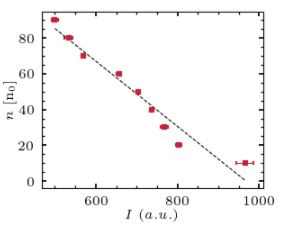
\includegraphics[width=0.8\textwidth]{figures/fig-s1_conc-calibration.jpg}
\caption[]{Concentration calibration.}
\end{center}
\label{fig:s1}
\end{figure}

\begin{figure}[ht]
\begin{center}
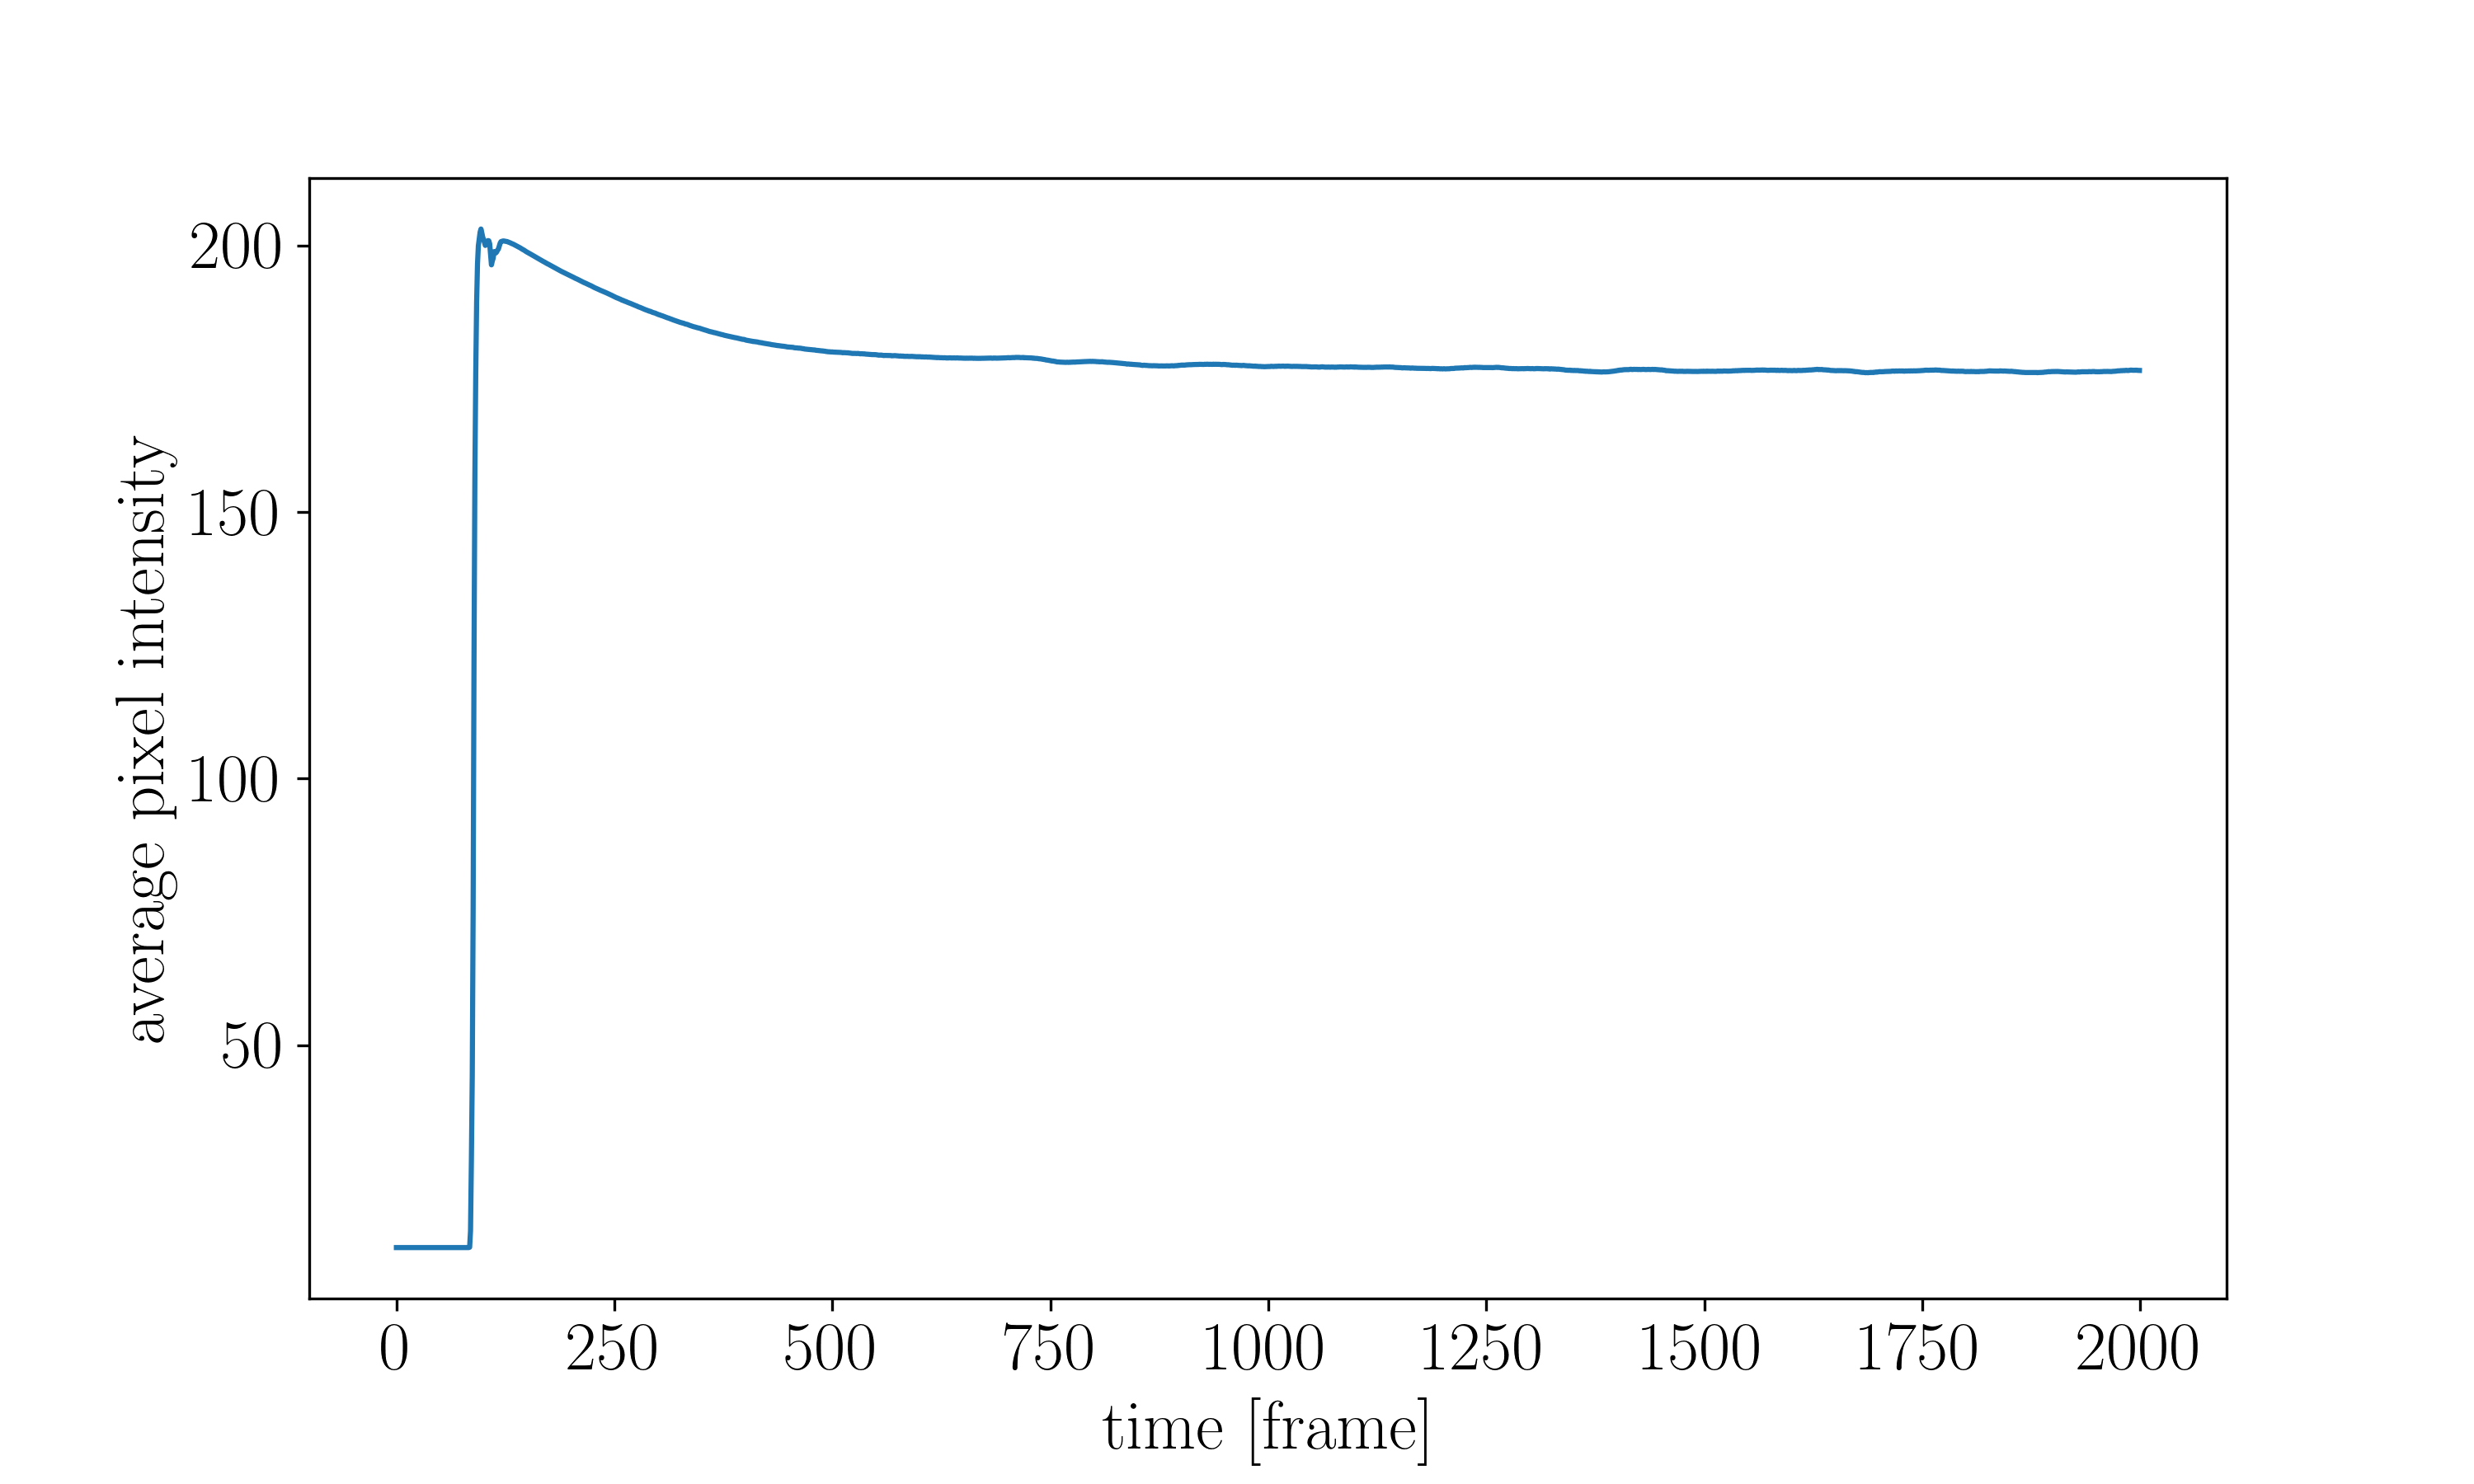
\includegraphics[width=0.8\textwidth]{figures/fig-s2_unstable-light.png}
\caption[]{unstable light}
\end{center}
\label{fig:s2}
\end{figure}

\begin{figure}[ht]
\begin{center}
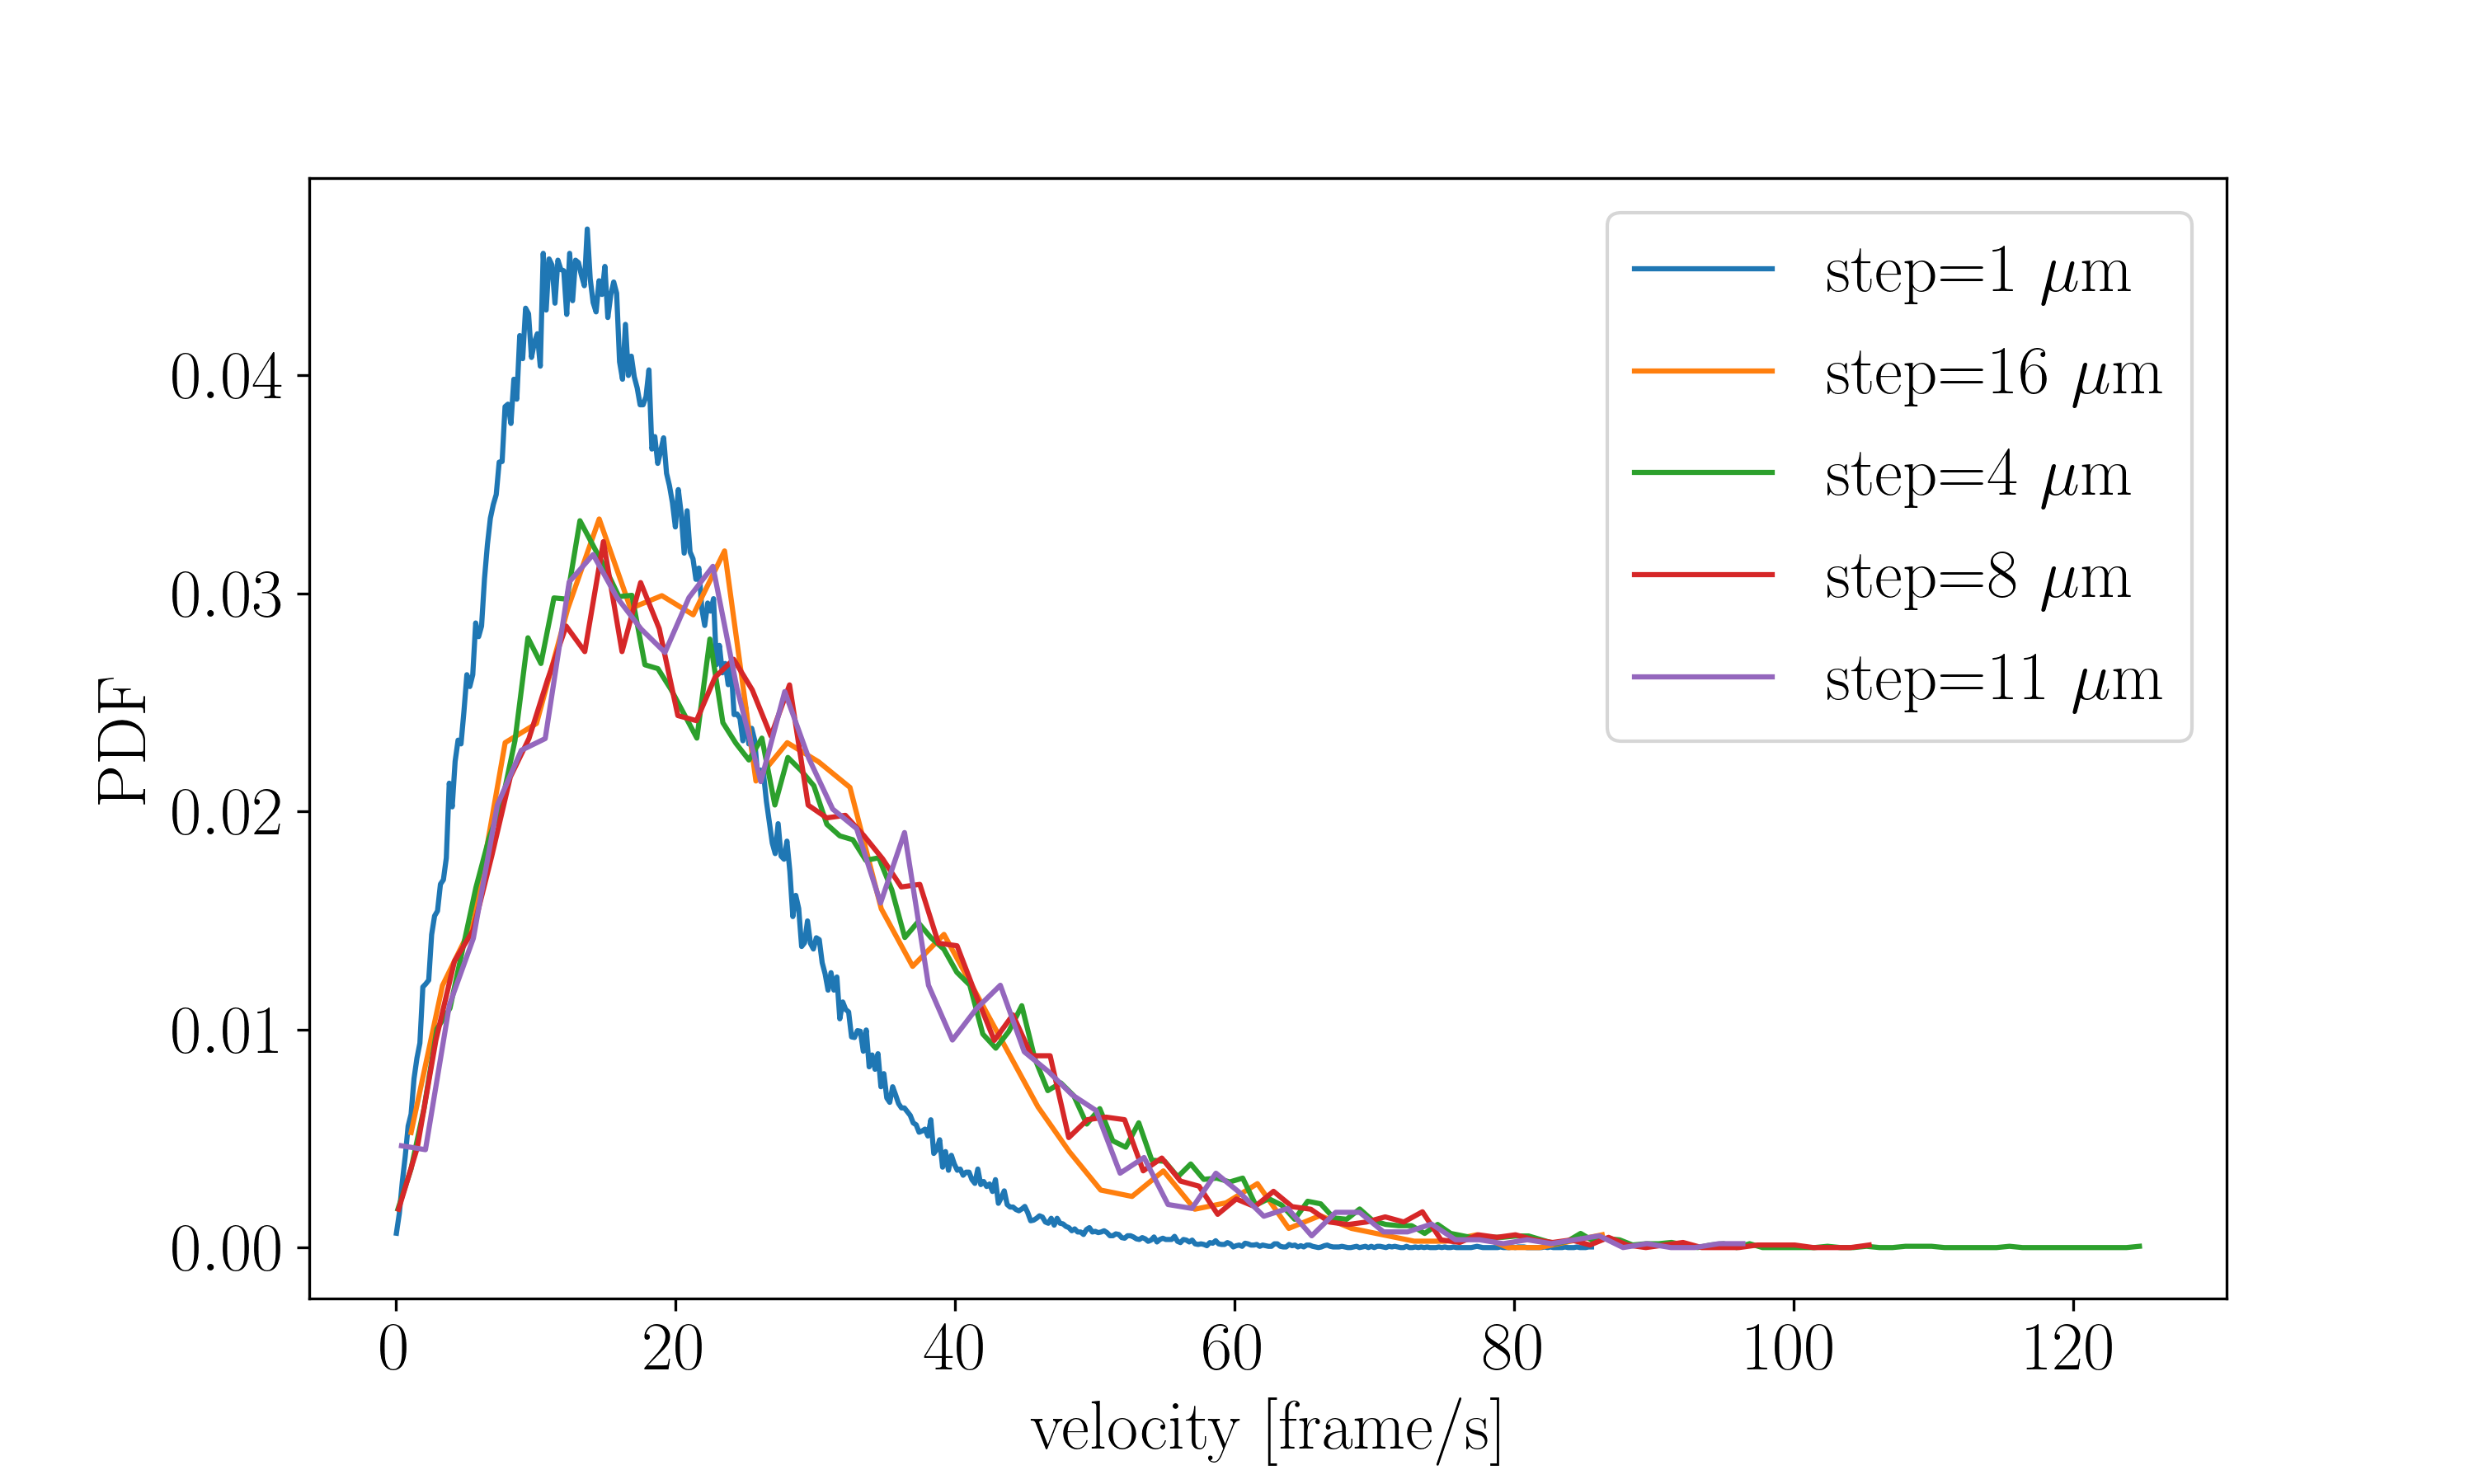
\includegraphics[width=0.8\textwidth]{figures/fig-s3_step-choice.png}
\caption[]{PIV step choice}
\end{center}
\label{fig:s3}
\end{figure}

\begin{figure}[ht]
\begin{center}
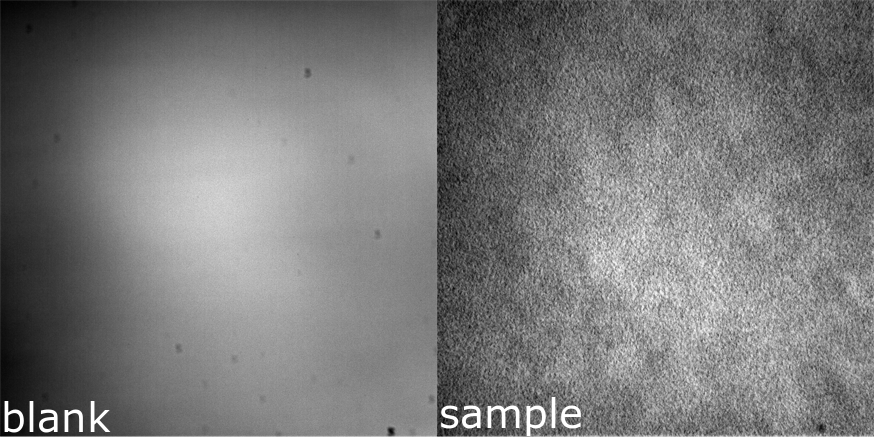
\includegraphics[width=0.8\textwidth]{figures/fig-s4_inhomogeneity.png}
\caption[]{inhomogeneity}
\end{center}
\label{fig:s4}
\end{figure}

\end{document}
